\subsection{Vzájomné interakcie}
\label{vzajomne_interakcie}
Ukázali sme implementáciu jednotlivých komponentov. Tie spolu komunikujú (\figurename{ \ref{idea}}) a vymieňajú si dáta. Táto podkapitola rozoberá implementačné detaily týchto procesov.  

\subsubsection{Passer - Server (šesťciferný kód)}
Teraz ukážeme príklad, ako server spracováva HTTP POST requesty od aplikácie Passer. Aplikácia odošle nový, šesťciferný, verifikačný kód spolu s heslami, ktoré používateľ cez Outsider odoslal. JSON štruktúra \texttt{SixdigitAuth} (spomíname v \nameref{passer}) môže vyzerať nasledovne: 
\newline
\lstset{literate={č}{{\v{c}}}1{ú}{{\'u}}1}
\begin{lstlisting}[basicstyle=\small]
{
    "deviceID":"F19494AE-555C-49FF-87DD-D94CA62D9634",
    "sixdigitCode":"791509",
    "passwordItems":[
        {
            "password":"password123",
            "id":"595C185D-DDF9-4BEA-A722-D383C75E5B33",
            "username":"username@example.com",
            "favourites":true,
            "group":1,
            "itemname":"Gmail účet",
            "url":"mail.google.com"
        },
    ],
    "bankCardItems":[],
    "otherItems":[],
    "timestamp":612273137.84391904
}
\end{lstlisting}
\leavevmode\newline
\indent V tejto ukážke si používateľ vybral možnosť verifikácie pomocou šesťciferného kódu a posiela jedno heslo - \textit{Gmail účet}. Server tieto dáta očakáva v tomto bloku kódu:
\newline
\begin{lstlisting}[language=Python, basicstyle=\small]
@app.route(`/sixdigit', methods=[`POST'])
def processSixDigitFromApp():
    incomingData = request.get_json()
    
    deviceID = incomingData[`deviceID']
    sixdigitCode = incomingData[`sixdigitCode']
    passwordItems = incomingData.get(`passwordItems')
    bankCardItems = incomingData.get(`bankCardItems')
    otherItems = incomingData.get(`otherItems')
\end{lstlisting}
\leavevmode\newline
\indent Server si uloží jednotlivé atribúty JSON štruktúry do premenných. Po spracovaní štruktúry nasleduje kontrola duplicít. Nasledujúci diagram ukazuje logiku ukladania dát do cache servera (pri šesťcifernom kóde): 
\newline
\begin{figure}[H]
  \centering
  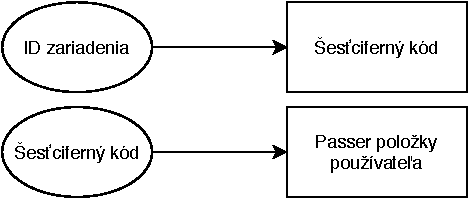
\includegraphics[width=10cm]{img/cache-diagram.pdf}
  \caption{Ukladanie dát do cache servera (šesťciferný kód).}
  \label{cache-diagram}
\end{figure}

Šesťciferný kód je namapovaný na ID zariadenia. Passer položky používateľa sú namapované na daný šesťciferný kód. Používame dve mapovania, lebo potrebujeme zaručiť, aby sa dvom rôznym používateľom (teda dvom rôznym ID zariadenia) nemohol vygenerovať rovnaký kód. Rovnako potrebujeme, aby jeden používateľ (teda jedno ID zariadenia) nebol kľúčom k viacero jednorázovým kódom (spomíname v \nameref{passer}). 

Pred zápisom novej verifikácie do cache najprv skontrolujeme, či nenastal jeden z dvoch konfliktných stavov, ktoré sme práve opísali.

Ako prvé zistíme, či zadaný šesťciferný kód existuje ako kľúč v cache. Ak áno, server vráti kód 409, čo znamená CONFLICT \cite{http_response}. Passer na to zareaguje opakovaním celej operácie.
\begin{lstlisting}[language=Python, basicstyle=\small]
    if cache.has(sixdigitCode):
        return 409
\end{lstlisting}

Druhá kontrola spočíva v tom, či pre daného používateľa už existuje nejaký šesťciferný kód. Ak existuje, musíme vymazať obe mapovania. 
\begin{lstlisting}[language=Python, basicstyle=\small]
    if cache.has(deviceID):
        userOldVerifData = cache.get(deviceID)
        cache.delete(deviceID)
        cache.delete(userOldVerifData)
\end{lstlisting}

Po týchto operáciách môže prebehnúť samotný zápis do cache. Pomocou \texttt{cache.set()} nastavíme mapovanie kľúč:hodnota a povieme, ako dlho má tento záznam existovať. Obe mapovania (\figurename{ \ref{cache-diagram}})  budú existovať na serveri po dobu dvoch minút.
\newline
\begin{lstlisting}[language=Python, basicstyle=\small]
    cache.set(deviceID,sixdigitCode,timeout=2*60)
    cache.set(sixdigitCode,[passwordItems, bankCardItems, otherItems, deviceID],timeout=2*60)
    return `server: ok', 201
\end{lstlisting}

Po úspešnej operácii Passer zobrazí používateľovi šesťciferný kód so zostávajúcim časom platnosti a inštrukciami.
\subsubsection{Webstránka - Server (šesťciferný kód)}
Používateľ už obdržal kód, ktorý môže použiť na webstránke na prístup k svojim položkám. Po jeho zadaní sa v JavaScript kóde webstránky spustí HTTP POST request na server. Posiela mu kód zadaný používateľom a čaká, ako odpovie server. Server sa snaží získať dáta namapované ku kľúču (\texttt{data = cache.get(sixdigitTyped)}). Kľúč je používateľom zadaný šesťciferný kód. 

Ak v cache neexistuje kľúč, ktorý by sa rovnal zadanému šesťcifernému kódu, premenná \texttt{data} bude \texttt{None}. Podľa toho sa mení návratová hodnota funkcie. 
\begin{lstlisting}[language=Python, basicstyle=\small]
    if data != None:
        cache.delete(sixdigitTyped)
        cache.delete(data[-1])
        response[sixdigitTyped] = data
        return response
    return `Wrong code'
\end{lstlisting}

Predtým, než vráti dáta späť webstránke, server vymaže záznamy v cache. Najskôr záznam pod kľúčom šesťciferného kódu, potom záznam pod kľúčom ID zariadenia. Následne vráti dáta.

Webstránka presmeruje používateľa na podstránku \texttt{.../passwords.html} a to nasledovne: \texttt{window.location.replace("passwords.html")}. Predtým ale potrebuje určitým spôsobom odovzdať podstránke dáta, ktoré práve od servera získala. JavaScript ponúka mnoho riešení, jedno z nich je local storage \cite{localstorage}.

\begin{sloppypar}
    Pomocou \texttt{window.localStorage.setItem("serverData",xhr.responseText)} uložíme do local storage odpoveď zo servera pod kľúč \texttt{serverData}. Následne sme schopní dáta z local storage vybrať, uložiť do premennej: \texttt{const serverData = window.localStorage.getItem("serverData")
    } a pracovať s nimi. Hneď po načítaní je potrebné vyčistiť local storage, inak by boli tieto dáta v pamäti aj počas ďalších sessions, ako uvádza \cite{localstorage}. Preto použijeme \texttt{localStorage.clear()}.
\end{sloppypar}

\subsubsection{Passer - Server - Webstránka (QR kód)}
Ako sme spomínali v sekcii \nameref{passer}, verifikácia pomocou QR kódu je špecifická. Počas nej prebieha interakcia so všetkými troma komponentmi (v úvodzovkách) naraz. 

\begin{sloppypar}
    Hneď po načítaní webstránky sa vygeneruje session id: \texttt{let sessionID = Date.now().toString(36) + Math.random().toString(36).substr(2, 5)}. Tento identifikátor vznikne operáciou zreťazenia aktuálneho času a náhodného čísla. Výsledný reťazec sa zakóduje do vygenerovaného QR kódu. Je zrejmé, že QR kód je zakaždým jedinečný, nakoľko obsahuje jedinečný session id reťazec.
\end{sloppypar}

Generovanie kódu je vďaka knižnici QRCode.js nasledovné: 
\newline
\begin{lstlisting}[language=JavaScript, basicstyle=\small]
function generateQRcode() {
    var qr = new QRCode(document.getElementById("qr-image"), {
        width: 120,
        height: 120,
        correctLevel : QRCode.CorrectLevel.L
    })
    qr.makeCode(sessionID)
}
\end{lstlisting}
\leavevmode\newline
\noindent V poslednom riadku si môžme všimnúť, že vytvárame QR kód s príslušnými dátami, teda s našim session id. To znamená, že ak niekto náš QR kód naskenuje, získa toto session id.

Vďaka tomuto reťazcu sa vie používateľ s Passerom verifikovať na webstránke. Princíp je teda podobný ako pri šesťcifernom kóde. Po naskenovaní v Passeri aplikácia vytvorí štruktúru, podobnú \texttt{SixdigitAuth}. Vyzerá takto:
\newline
\begin{lstlisting}[language=Swift, basicstyle=\small]
struct QRAuth: Codable {
    let sessionID: String
    let passwordItems: [PasswordItem]?
    let bankCardItems: [BankCardItem]?
    let otherItems: [OtherItem]?
}
\end{lstlisting}
\leavevmode\newline
\noindent Atribút \texttt{sessionID} je session id naskenovaná z QR kódu. Ďalšie atribúty sú polia Passer položiek, ktoré sa spolu so \texttt{sessionID} odošlú na server rovnakým spôsobom, ako pri šesťcifernom kóde. Pri QR verifikácii je len jedno mapovanie v cache servera: 
\newline
\begin{figure}[H]
  \centering
  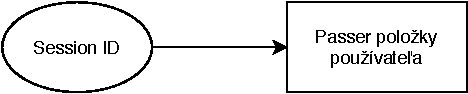
\includegraphics[width=10cm]{img/cache-diagramQR.pdf}
  \caption{Ukladanie dát do cache servera (QR kód).}
  \label{cache-diagramQR}
\end{figure}

Medzičasom webstránka cyklicky kontroluje server, či už existuje v cache kľúč s daným session id. Aby sa zabránilo preťaženiu, robí tak iba raz za sekundu. Akonáhle webstránka dostane pozitívnu odpoveď a dáta používateľa, požívateľ je presmerovaný na podstránku \texttt{.../passwords.html}. Operácie, ktoré vykonáva server s verifikačným reťazcom sú takmer totožné s operáciami pri overovaní šesťciferného kódu.

Ukážeme ešte spôsob cyklického kontrolovania servera na strane webstránky:
\newpage
\begin{lstlisting}[language=JavaScript, basicstyle=\small]
setInterval(function() {
    let xhr = new XMLHttpRequest()
    xhr.open("POST", "https://api-passer.herokuapp.com/verifyQRfromwebsite", true)
    xhr.setRequestHeader("Content-Type", "application/json")
    xhr.onreadystatechange = function () {
        if (xhr.readyState === 4 && xhr.status === 201) {
            window.localStorage.setItem("serverData",xhr.responseText)
            window.location.replace("passwords.html")
        }
    }
    let data = { "sessionID": sessionID }
    let jsonData = JSON.stringify(data)
    xhr.send(jsonData)
}, 1000) 
\end{lstlisting}
\leavevmode\newline
\indent \texttt{XMLHTTPRequest()} sa spúšťa až exekúciou riadku \texttt{xhr.send()} v dolnej časti kódu. Podobná logika requestov sa vykonáva aj v jazyku Swift, na ktorom je postavený Passer.

\leavevmode\newline
\indent Toto sú všetky interakcie našich troch komponentov, ktoré vystihujú myšlienku celej práce. Týmto spôsobom sme docielili prístup používateľa k svojim dátam aj mimo ekosystém.